\chapter{Introduction}\label{chap:intro}
\newcommand{\ignore}[1]{}
\ignore{Write this chapter LAST. Should be 5 to 10 pages. This chapter provides a quick summary of the
essential contents of the research project, principal results and contents of the report. The target
audience is members of the jury who do NOT have time to completely read all 21 reports, as well
academic members of other juries who wish to compare this work to other works.}

\section{Background}
\ignore{This is a generic title. Replace it with an actual title that describes the context of the work.
Short .5 page summary of the technological context of the work and why it is interesting or important}

3D animation can be a painstakingly tedious activity. To create a desired animation, animators go through the long process of keyframing. Keyframes are set positions that define the start and end points of a movement, sequences of poses which are transformed in time. Typically, animators assign poses to certain frames over time, so that in-between motions can be generated by a computer. To get an accurate animation, artists usually must assign many keyframes, then spend time adjusting and editing them to be more precise. The fact that industry professionals take so much time and effort to do this shows that for an amateur or untrained artist, creating \textit{good} 3D animation is close to impossible. 

In \autoref{fig:keyframes}, the character has keyframes attached to it on the timeline, shown in the yellow box, which represent its various positions and rotations in time.

%\begin{wrapfigure}{R}{0.5\textwidth}
\begin{figure}[h!]
\centering
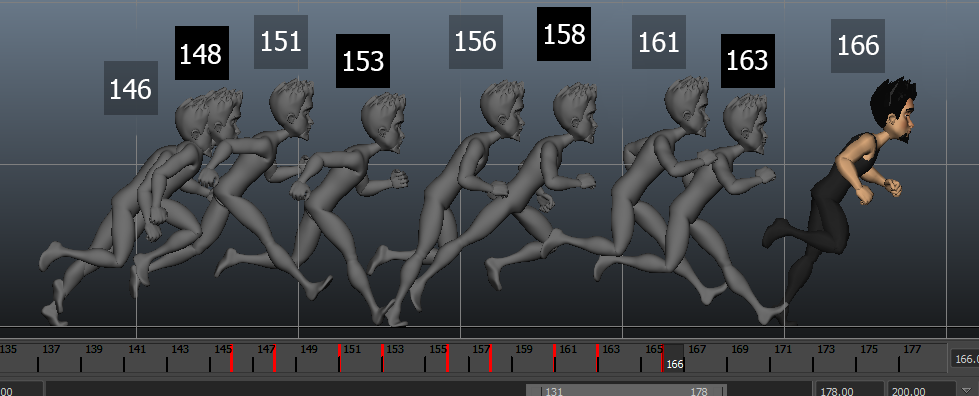
\includegraphics[scale=0.7]{img/newrunningposes}
\caption{Example of keyframing in Autodesk Maya. Red lines on the timeline indicate keyframes for the character.}
\label{fig:keyframes}
\end{figure}
%\end{wrapfigure}

\section{Problem Statement}
\ignore{This is a generic title. Replace it with an actual title that describes the context of the work.
Approx .5 to 1 page description of the research problems that was addressed and what was required to address it.}

Among the most complicated characters to animate in 3D animation are humanoid characters. To ease this task, animators create a skeleton for their character called a \textbf{rig}, that consists of joints connected by rigid links (bones) to give a structure to the character. Humanoid rigs can range in complexity from somewhat simple to extremely complicated depending on the amount of detail desired by the user. The structure is a hierarchy of joints that can also be seen as a tree with a root, which in the humanoid case, is usually the pelvis. The leaf nodes of this tree, which are loacted at the maximal parts of the body, are called \textbf{end effectors}. Leaf nodes come at the end of a \textbf{kinematic chain}, which can be followed back up to the root.


\begin{figure}[h!]
	\centering
        \begin{subfigure}[b!]{0.55\textwidth}
        	\centering
                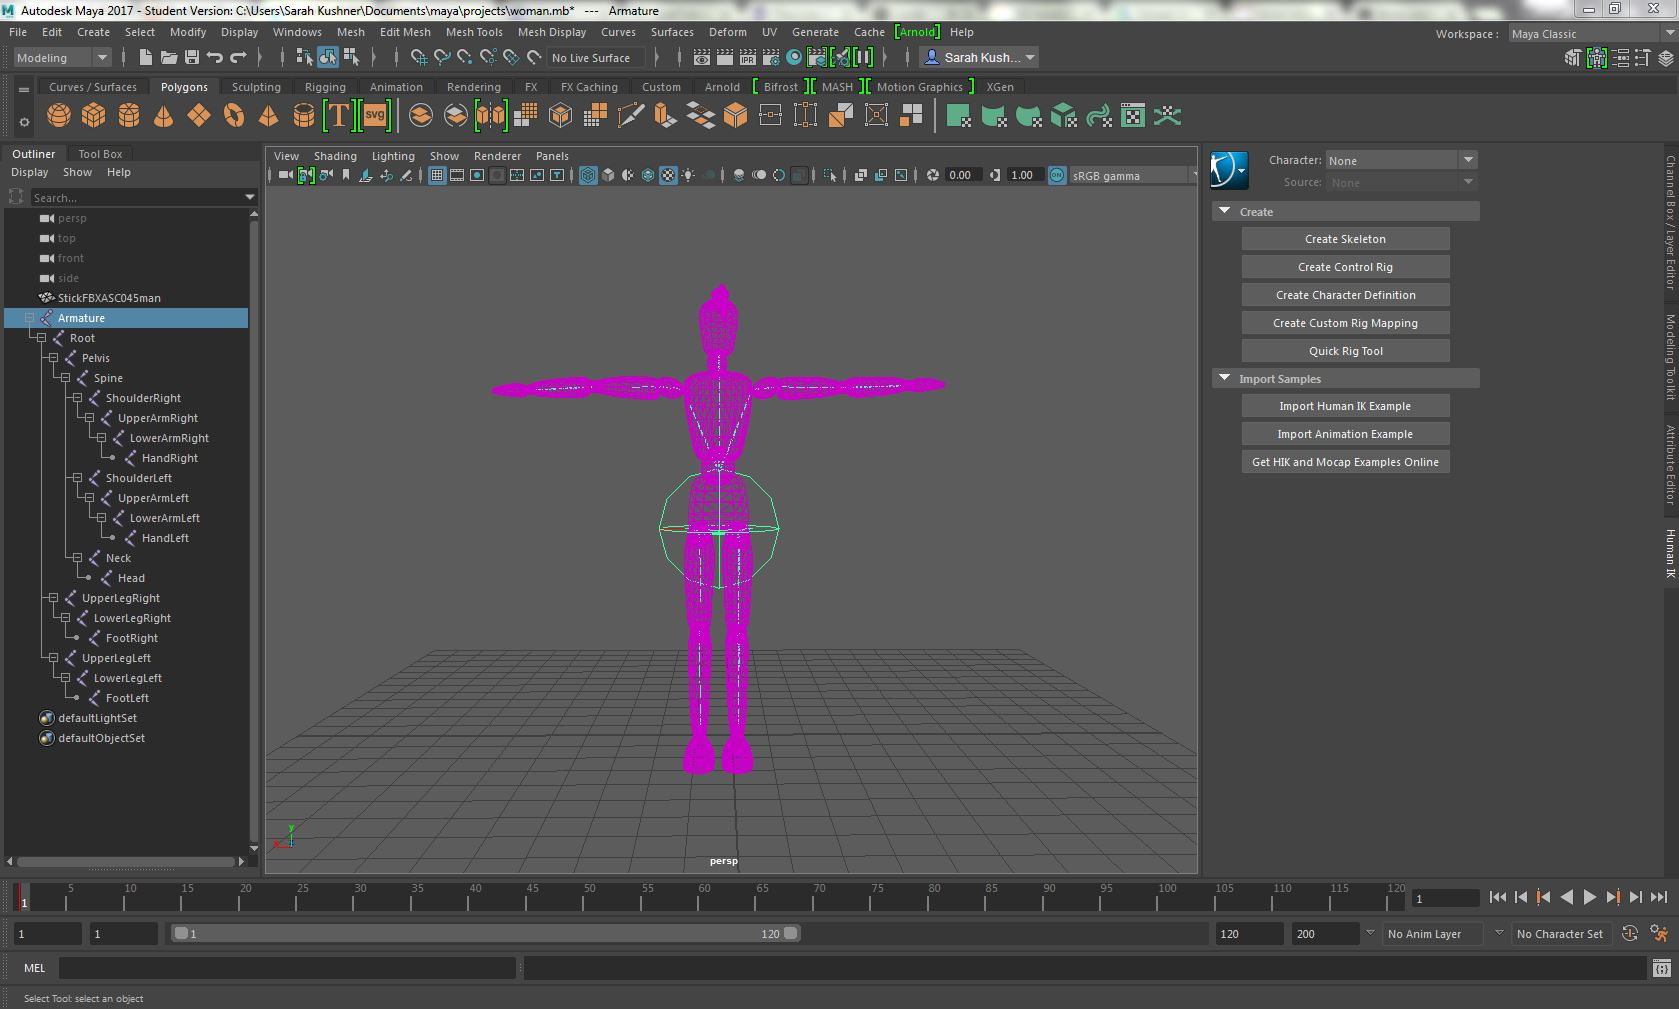
\includegraphics[width=\linewidth]{img/skeleton}
                \caption{Example of a humanoid skeleton.}
                \label{fig:skeleton}
        \end{subfigure}
        \quad
        \begin{subfigure}[b!]{0.4\textwidth}
        	\centering
                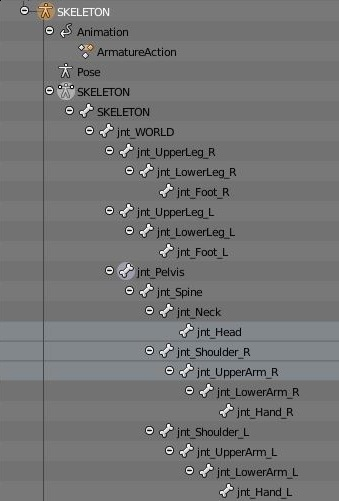
\includegraphics[width=\linewidth]{img/skeleton_hierarchy}
                \caption{The hierarchy of joints corresponding to the skeleton.}
                \label{fig:hierarchy}
        \end{subfigure}%
	\caption{Humanoid skeleton shown in Blender.}
	\label{fig:rig}
\end{figure}

\subsection{Kinematics}
Forward and inverse kinematics are two general animation methods used mainly in situations in which articulated characters need to move according to some contraints. In order to animate this structure successfully, controls are added that allow for forward and inverse kinematics. These controls help the animator move the character into poses that will then act as keyframes.

\textbf{Forward kinematics} (FK) is a method of calculating the position and orientation of the end effector (i.e. a hand or foot) given the positions and angles of the joints higher up in the chain all the way to the root. 

\textbf{Inverse kinematics} (IK) is the method opposite of forward kinematics. That is, the goal is to calculate the angles and positions of joints in the chain, given the angle and position of the end effector. This goal is much harder to reach, seeing that more information needs to be calculated than is given. This problem is underconstrained. There can be more than one correct configuration that satisfies the constraints or there can even be no viable configurations. Many IK algorithms exist to calculate joint angles and positions, which will be explained further in \autoref{chap:issues}.

Inverse kinematics are clearly more desirable for an animator since it is easier and faster to pose a character and have the joint angles automatically computed than it is to manipulate the character's joints directly.

\subsection{The Line of Action}
In practice, both forward and inverse kinematic controls is used in combination. Although this is the standard, even manipulating controls can be time-consuming. Sketch-based interfaces have started to become a plausible option for both animators and those with less experience. Many papers have been authored dealing with the sketch-based posing of a single humanoid character, discussed later in \autoref{chap:sota}. However, the animation of multiple characters comes with its own unique set of challenges as well. The problem is discovered when humanoid characters interact, namely when they are in close proximity to each other or when they touch each other.

The line of action is the concept of imagining a line that extends through the character's main action. It is commonly used by cartoonists in gesture drawings and the early stages of storyboarding to accentuate the motion and shape of the character. These lines are often dramatic in shape but smooth and simple in quality, usually containing only one or two extrema. The line of action goes through the majority of a character's body or through a part of the body and has a clear direction. See \autoref{fig:lines}.

\begin{figure}[h!]
	\centering
        \begin{subfigure}[b!]{0.45\textwidth}
        	\centering
                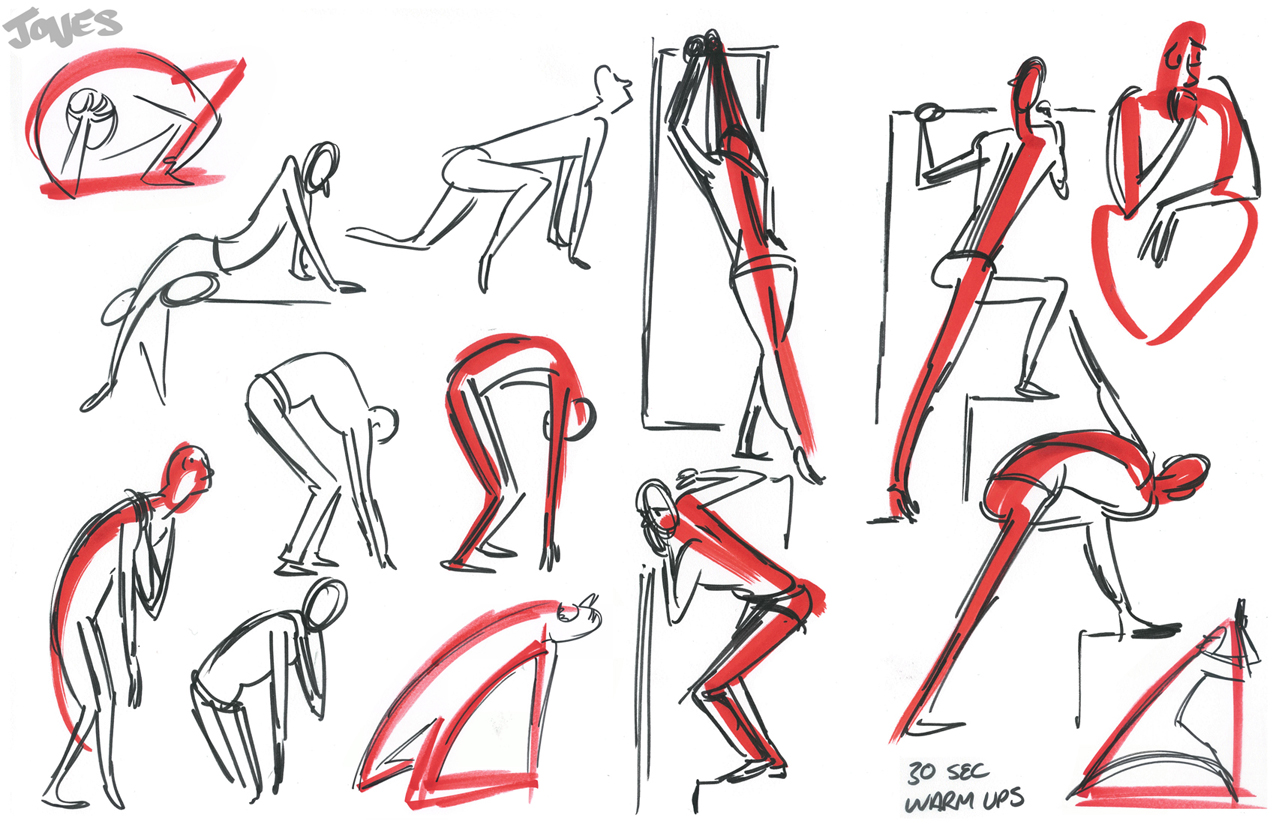
\includegraphics[width=\linewidth]{img/cartoon}
                \label{fig:gesture}
        \end{subfigure}
        \quad
        \begin{subfigure}[b!]{0.45\textwidth}
        	\centering
                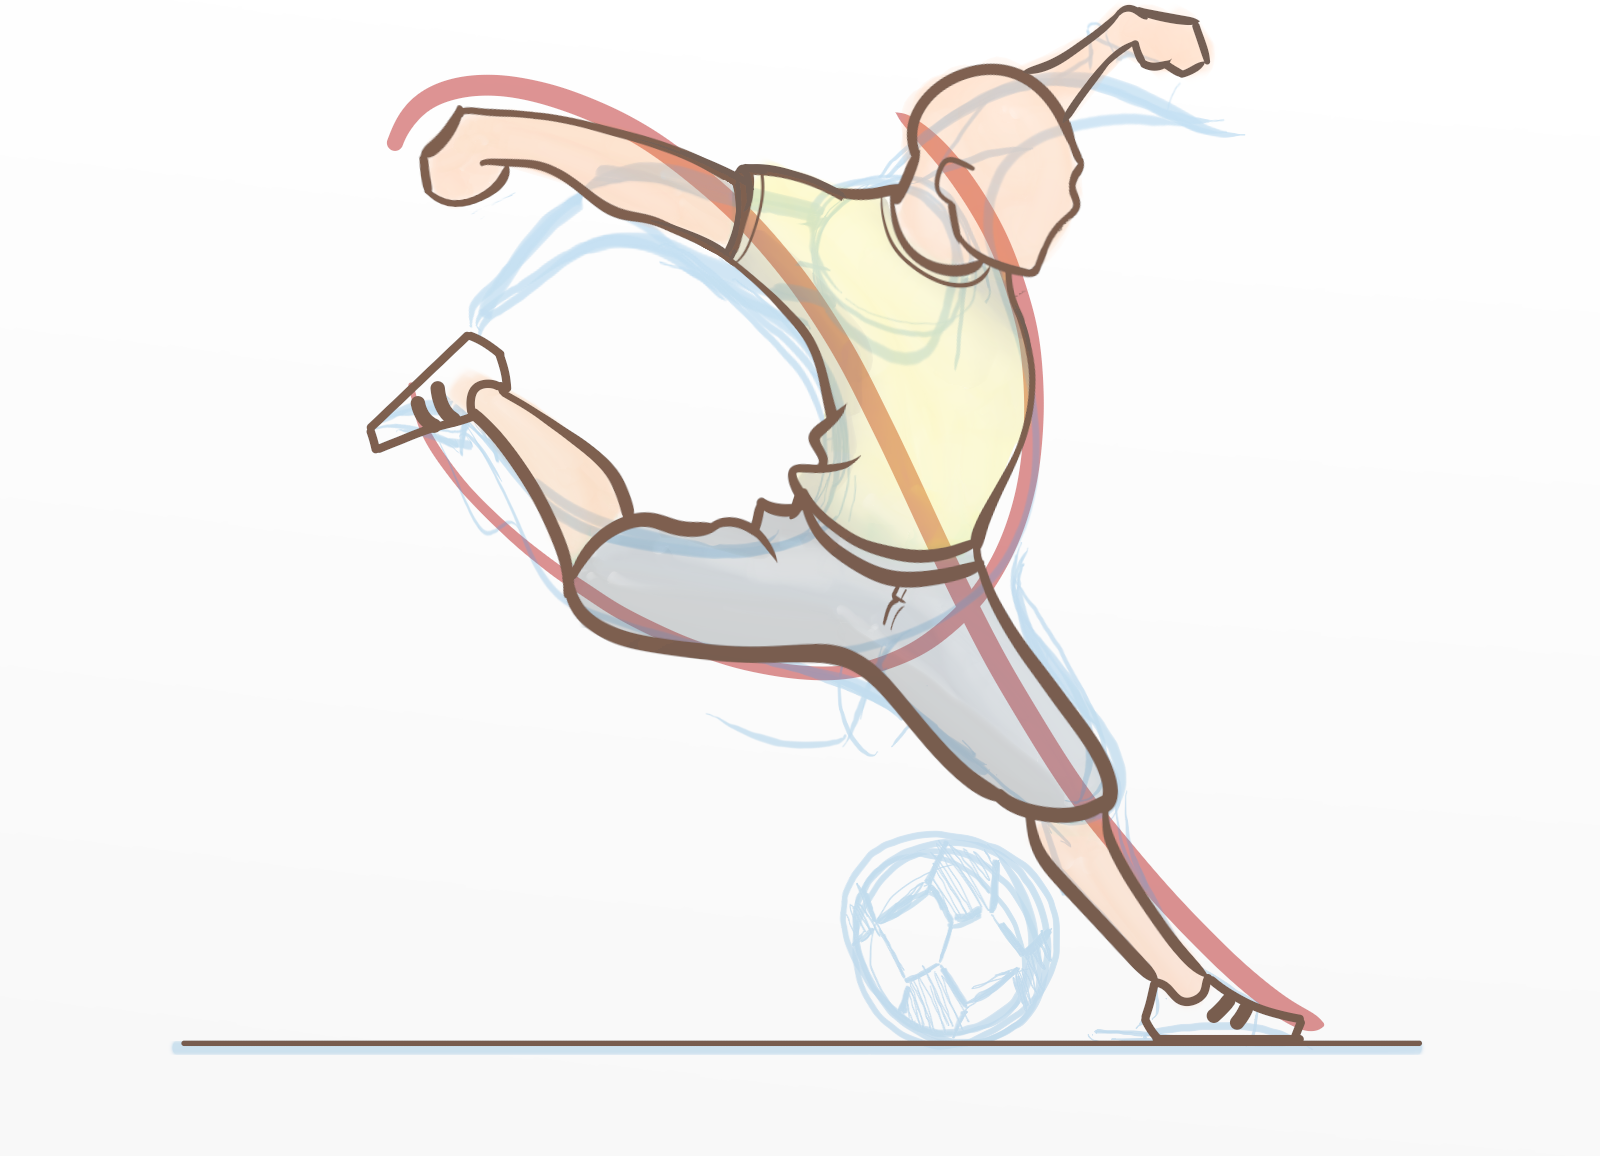
\includegraphics[width=\linewidth]{img/kick}
                \label{fig:kick}
        \end{subfigure}%
        \caption{Line of action examples.}
	\label{fig:lines}
\end{figure}

The line of action has many advantages, including FILL THIS IN. This concept transfers over to sketch-based posing very intuitively. Shown in \autoref{chap:issues}, posing with the line of action works incredibly well for a single character. It provides a more straighforward and quick way of animating a single humanoid character. Extending the line of action to more than one character is nontrivial. Left on its own, many undesirable effects like collisions make the tool frustrating to use, rather than convenient. 

\section{Proposed Approach}
\ignore{This is a generic title. Replace it with an actual title that describes the context of the work.
Approx 1 to 2 page description of the scientific approach or approaches to a solution and how it was investigated and evaluated. Present a summary of the principal results obtained.}

The use case for this research in multi-character animation is a dancing couple. There are many combinations of poses a human can be in, let alone two humans \textit{and} the two humans interacting. Specifically, a clip from the film ``The Band Wagon'' (\citep{thebandwagon1953}) was used to observe the common motions and poses in a dancing couple.



Using the previous work (\citep{guay2013line}, \citep{guay2015adding}, and \citep{guay2015space}), already in the process of being developed by the IMAGINE team, I extend the functionality of the line of action to be applied to multiple characters. Their software acted as the baseline with which to compare the new features. Baseline poses and animations were made by taking important keyframes from the film clip to recreate in their software. The amount of time spent running the program, the number of clicks, and number of lines drawn were recorded.

Since characters' skeletons are essentially trees, a novel approach to solving this problem was combining these kinematic trees into one in a new data structure with special attributes for posing and animating. An interesting way to evaluate this notion of animating a combined character was to, again, reproduce the same poses and animations as in the baseline, but this time using the new structure instead.

Results to come I hope

\section{Contents of this report}
\ignore{Approx .5 page per chapter. Summarize the contents of the subsections of each chapter. Give the
topics addressed and summarize what is written in each chapter.}

In the following chapter (\autoref{chap:sota}), I cover the state-of-the-art for this particular problem. I discuss a brief history of dance notation -- how choreographers and dancers use sketching on paper to brainstorm and communicate their ideas of motion, formation, and pose of dance. Then I will talk about the existing sketch-based systems used for posing articulated characters, covering the benefits and limitations of each. A sizeable portion of my work has had to do with kinematic trees and graph data structures, so I will go into a few important graph theory algorithms. Generating animation from existing data is also a widely relevant topic to my work. So, I also describe previous research regarding that.

In \autoref{chap:issues}, the fundamentals of character animation are more closely examined. (more to come when I actually write it...)

\autoref{chap:implementation} covers exactly how a solution was reached and what it entails. (more to come when I actually write it...)

\autoref{chap:results} is where I go over the methods of validating our solution. (more to come when I actually write it...)

Discussion of the lessons learned during this project and the concluding thoughts on the process are explored in \autoref{chap:discussion} and \autoref{chap:conclusion}, respectively. (more to come when I actually write it...)

